\documentclass[../../main.tex]{subfiles}

\graphicspath{{images/Steuerungssoftware/}{../../images/Steuerungssoftware/}}
\begin{document}
\subsection{Steuerungssoftware} \label{it_steuerungssoftware}
In diesem Kapitel wird auf die Implementierung der technischen Komponente 'Steuerungssoftware' eingegangen. Auch wird ein Augenmerk auf unsere Middleware 'ZeroMQ' und die Datenserialisierung mittels 'Protobufers' gelegt. Die Steuerungssoftware befindet sich im Mittelpunkt der Applikation und kann somit auch als Herzstück bezeichnet werden. Sie orchestriert die verschiedenen Module, damit ein funktionierendes Zusammenspiel ermöglicht wird und der Applikationsablauf geschmeidig durchlaufen wird.

\subsubsection{Anforderung}

\begin{itemize}
    \item Korrekte Ausführung des PREN-Ablaufs
    \item Robust
    \item Ausführung einzelner Module
\end{itemize}

\subsubsection{Lösung}
Die Steuerungssoftware wird wie in PREN beschrieben mittels der Middleware Technologie 'ZeroMQ' und 'Protobufers' unterstützt. Die Steuerungssoftware selbst erbt wie alle anderen Module auch von der Basisklasse 'App', dazu später mehr. Solange die Steuerungssoftware läuft wartet sie auf ein Startsignal, welches den Applikationsablauf in Gang setzt.

\subsubsection{Technologien / Aufbau}
Einblick in verwendete Technologien, sowie ein Überblick über Programmstruktur und Aufbau der Middleware. 

\textbf{ZeroMQ} \\
ZeroMQ 

\textbf{Protocol buffers} \\
Protocol buffers, auch Protobuf, ist ein von Google entwickeltes Protokoll zum Senden und Empfangen von serialisierten und deserialisierten Daten über verschiedene Dienste. Google's Design Ziel für Protobuf liegt darin kleiner, einfacher und schneller als XML zu sein. Unterstützt werden alle häufig verwendet Sprachen wie: Python, Java, Objective-C, C\# und andere.

\textbf{Beispiel Protobuf:}
\lstinputlisting{../src/raspi/pb/direction.proto}
Man sieht nun, dass eine 'Direction' Mitteilung definiert wird. Diese hat ein String Attribut, welches direction heisst. Mit dieser Definition wird mithilfe eines 'protobuffer compiler' Code generiert. Dieser kann die definierte Message Serialisieren und Deserialisieren.

\pagebreak

\textbf{Beispiel Generierung für Python:}
\begin{lstlisting}
    protoc -I=pb --python_out=pb pb/direction.proto
\end{lstlisting}
Mithilfe von diesem Beispiel wird die Protobuf Definition (direction.proto) zu Python Code generiert.

\textbf{Beispiel Generierter Python Code:}
\lstinputlisting[language=Python]{../src/raspi/pb/direction_pb2.py}
Das generierte Python File, welches mithilfe des 'protobuffer compiler' erzeugt wurde.

\vspace{1cm}

\textbf{Protobuf Nachrichten} \\
Eine Auflistung aller verwendeter Protobuf Nachrichten, welche über die Middleware gesendet werden.
\begin{table}[H]
  \begin{tabular}{lll}
  \hline
  \textbf{Nachricht} & \textbf{Bezeichner} & \textbf{Datentyp} \\ \hline
  Acceleration & x & Integer32bit \\ 
   & y & Integer32bit \\
   & z & Integer32bit \\ \hline
  CraneCommand & command & Integer32bit\\ \hline
  Cube & state & Integer32bit\\ \hline
  Current & current & Integer32bit\\ \hline
  Direction & direction & String\\ \hline
  Distance & distance & Float\\ \hline
  Heartbeat & component & String\\ 
   & status & String\\ \hline
  MoveCommand & speed & Integer32bit\\ \hline
  NumberDetection & number & String\\ \hline
  Speed & speed & Integer32bit\\ \hline
  SystemCommand & command & String\\
   & phases & Map<String, Boolean>\\ \hline
  SystemStatus & phase & String\\
   & message & String\\ \hline
  \end{tabular}
\end{table}

\pagebreak


\textbf{Kommunikationsmodule} \\
\begin{figure}[H] \centering
  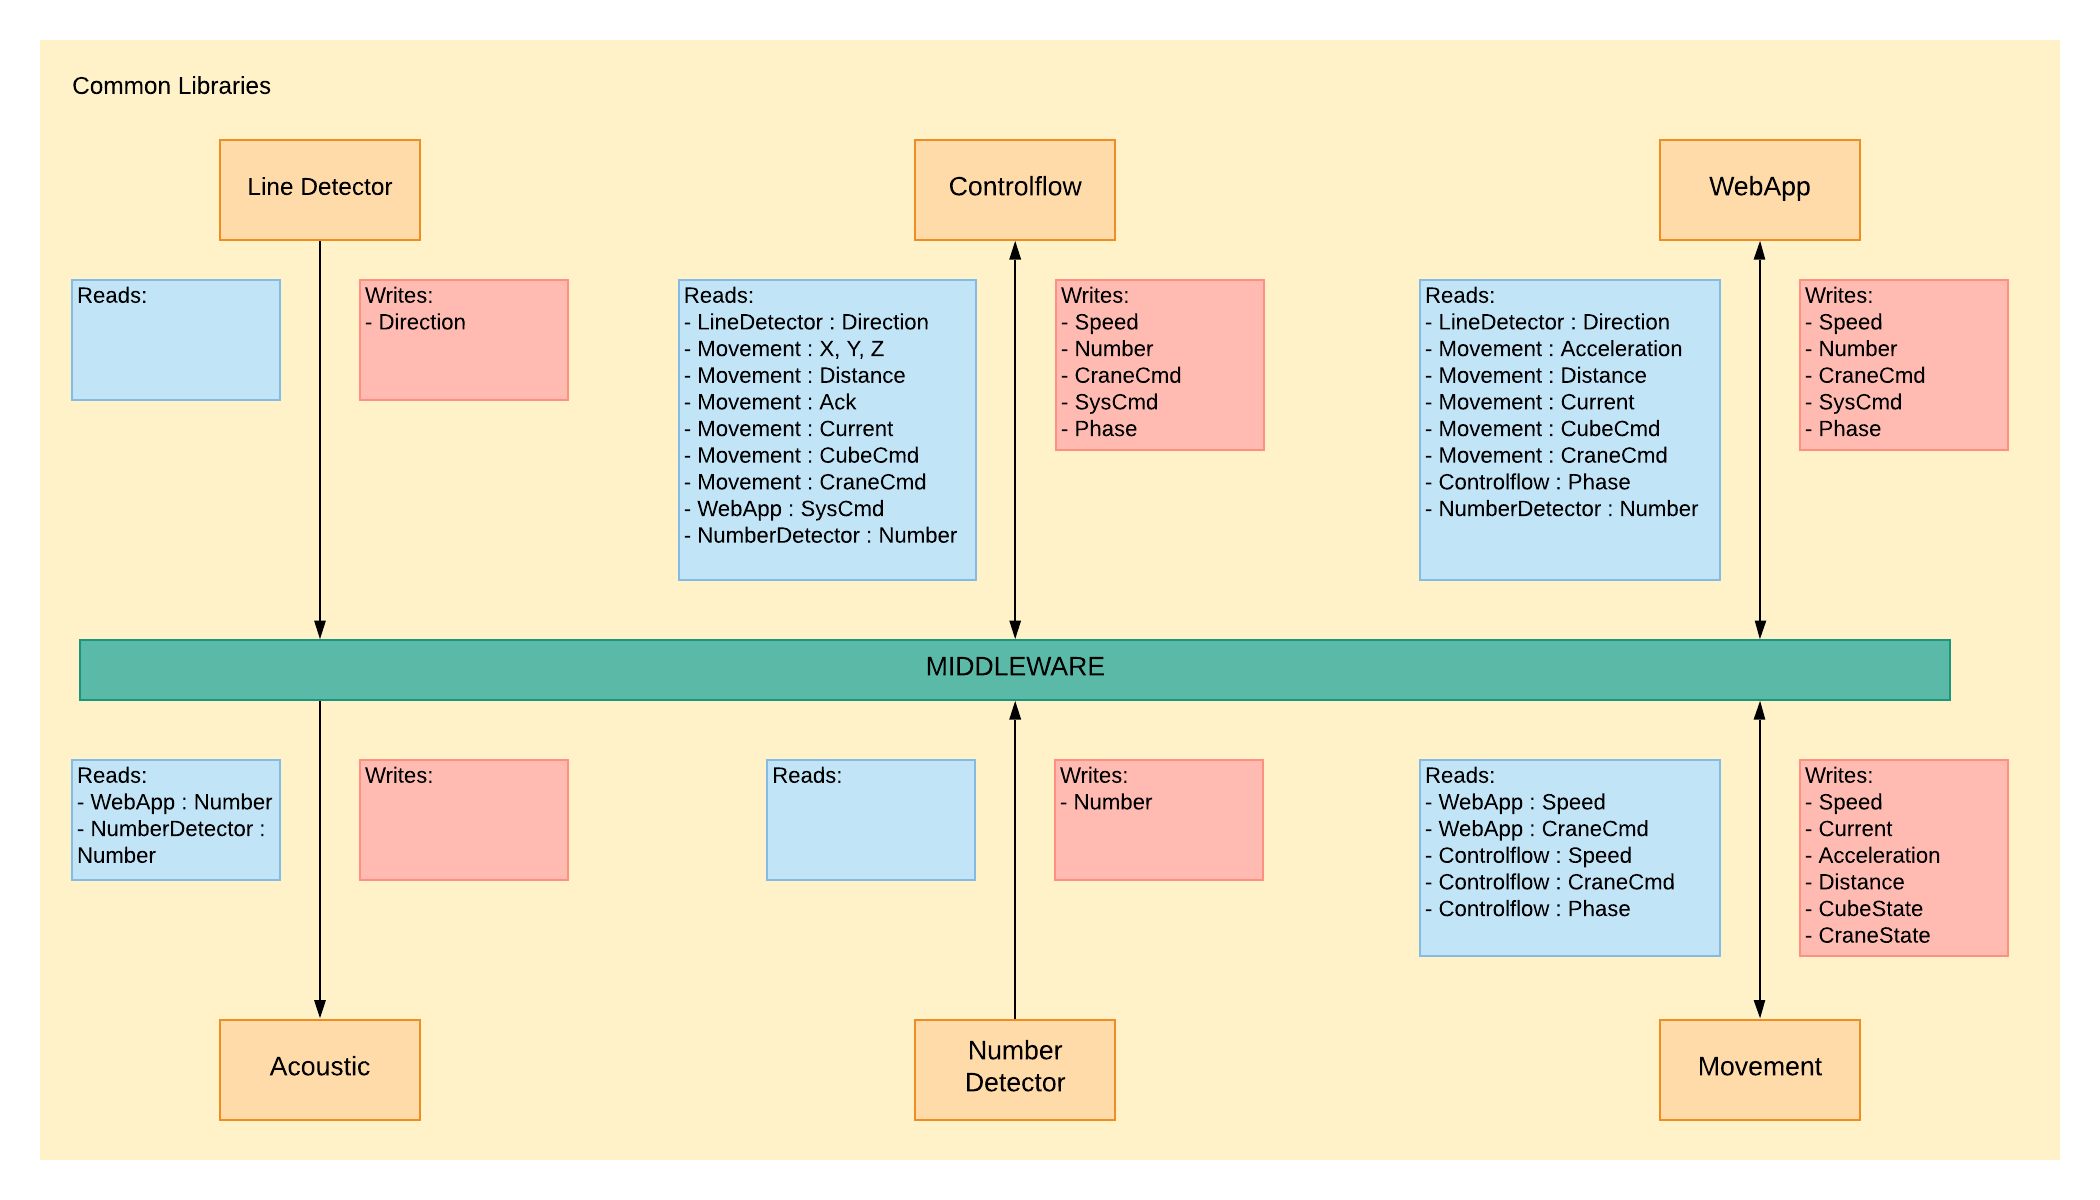
\includegraphics[width=1\textwidth]{Architektur}
  \caption{Kommunikation}
  \label{fig:Kommunikation}
\end{figure}
Das Senden / Empfangen der Hearbeats wurde in obigem Diagram bewusst weggelassen, die Hearbeats haben keinen direkten Einfluss auf das Verhalten der Applikation und sind somit für die Steuerung irrelevant.

\textbf{Heartbeat} \\
Der Heartbeat spiegelt den Zustand des Moduls wieder, welches ihn sendet.
Jedes Modul besitzt einen Hearbeat, welches in regelmässigen Abständen gesendet wird. Ein Modul kann folgende Zustände annehmen:
\begin{table}[H]
    \begin{tabular}{ll}
    \hline
    Starting & Während der Initialisierungsphase des Moduls \\ \hline
    Running & Solange das Modul läuft\\ \hline
    Error & Sobald ein Fehler gemeldet wird oder das Modul keinen Hearbeat mehr sendet\\ \hline
    Finished & Nach Abschluss seiner eigentlichen Tätigkeit\\ \hline
    \end{tabular}
\end{table} 
Folgende Module werden überwacht:
\begin{table}[H]
    \begin{tabular}{ll}
    \hline
    Line Detector & Liest die Richtung der aufkommenden Gleise während der Fahrt \\ \hline
    Number Detector & Liest die Nummern während der Fahrt\\ \hline
    Movement & Liest Geschwindigkeit und regelt die momentane Geschwindigkeit anhand dessen\\ \hline
    Acoustic & Gibt die eingelesene Nummer akustisch wieder\\ \hline
    Control Flow & Regelt den Ablauf der verschiedenen Phasen \\ \hline
    \end{tabular}
\end{table}

\pagebreak

\textbf{Codestruktur (Basisklasse)} \\
Alle Module erben von der Basisklasse.\\
\begin{lstlisting}
  class Buzzer(base_app.App):
    def __init__(self, *args, **kwargs):
        super().__init__("Acoustic", self.acoustic_loop, *args, **kwargs)
\end{lstlisting}
Module teilen sich die Eigenschaft einer nebenläufigen Methode, welche Nachrichten aus der Middleware liest. Somit wurde diese Funktionalität in eine Basisklasse ausgelagert. Die Basisklasse führt die Methode aus bis die Applikation beendet wird.\\
\begin{lstlisting}
  def run(self):
  try:
      while not self.stopped:
          self.loop(self.args, self.kwargs)
  except ProgramKilled:
      self.stopped = True
\end{lstlisting}
Das Auslesen, Senden und Verarbeiten der Daten erfolgt in jedem Modul separat.

\subsubsection{Entwicklungsablauf}
Bevor mit dem Ablauf begonnen wurde, stellten wir sicher, dass die einzelnen Module einwandfrei funktionieren, um Probleme während der Fahrt auf ein Minimum zu begränzen. Die Steuerungssoftware wurde gegen Ende von PREN2 entwickelt und getestet. \\

Die Architektur war schon zu Beginn von PREN2 vefügbar und lauffähig. Während der Entwicklung von PREN2 wurde die Middleware kontinuierlich erweitert. Gegen Ende gab es ein Refactoring der Middleware Schnittstelle, wobei das Abonnieren von Nachrichten um ein Vielfaches einfacher wurde.

\subsubsection{Testing}
Während dem Testen kamen verschiedene Probleme auf. Ein grosser Blocker war das Fahren selbst. Der Zug blockierte (bei niedrigen Geschwindigkeiten) und entgleiste oft. Dies erschwerte das Testen des kompletten Ablaufs erheblich. Das Problem wurde von unseren Mechanikern rasch beseitigt. \\

Bei der Ausgabe eines akustischen Signals wurde festgestellt, dass die Kabel falsch verbunden wurden. Auch war die Ausgabe des Signals nicht wie erwartet, was ebenfalls behoben wurde. \\

Die Kamera wackelte während der Fahrt stark, wobei die Bilder verwackelt wurden. Mithilfe eines Gummiuntersatzes an der Kamerahalterung wurde dem Wackeln entgegengewirkt. Das Ergebnis waren einiges schärfere Bilder.

\end{document}